\documentclass{beamer}
\usepackage{graphicx}
\usepackage{xcolor}
\usepackage{tikz}
\usepackage{amsmath}

\definecolor{purpleblue}{RGB}{80, 80, 180}
\definecolor{novelPurple}{RGB}{98, 54, 255}
\definecolor{softPurple}{RGB}{180, 170, 255}
\definecolor{softGray}{RGB}{235, 235, 245}
\definecolor{lightText}{RGB}{90, 90, 110}

\usetheme{Madrid}
\usecolortheme{dolphin}
\graphicspath{{static/course_materials/}{static/hard/}{./}}

\setbeamerfont{title}{size=\Large,series=\bfseries}
\setbeamerfont{frametitle}{size=\LARGE,series=\bfseries}
\setbeamercolor{frametitle}{fg=white, bg=novelPurple}
\setbeamercolor{title}{fg=white, bg=purpleblue}

\title[SAT Hard Question 2]{\textbf{SAT Hard Question\\ Set 2}}
\author{\textbf{Jack Zeng}}
\institute{\textcolor{white}{\textbf{Novel Prep}}}
\date{\today}

\begin{document}

\begin{frame}
    \titlepage
    \vfill
    \begin{flushright}
        \textcolor{purpleblue}{\Huge \textbf{Novel Prep}}
    \end{flushright}
\end{frame}

\begin{frame}
    \begin{tikzpicture}[remember picture, overlay]
        \shade[top color=softPurple, bottom color=softGray]
            (current page.north west) rectangle (current page.south east);
        \node[align=center] at (current page.center) {
            {\Huge\bfseries\textcolor{purpleblue}{Novel Prep}} \\[0.5cm]
            {\Large\itshape\textcolor{lightText}{Phase 2 · Hard Question Practice}}
        };
    \end{tikzpicture}
\end{frame}

\begin{frame}{Overview}
    \tableofcontents
\end{frame}

\begin{frame}
\section{Hard Question Set 2}
    \begin{tikzpicture}[remember picture, overlay]
        \shade[top color=softPurple, bottom color=softGray]
            (current page.north west) rectangle (current page.south east);
        \node[align=center] at (current page.center) {
            {\LARGE\bfseries\textcolor{purpleblue}{Hard Question Set 2}} \\[0.5cm]
            {\Large\itshape\textcolor{lightText}{9 SAT-style challenge problems}}
        };
    \end{tikzpicture}
\end{frame}

% --- Question 1 ---
\begin{frame}{Question 1}
\small
\begin{center}
    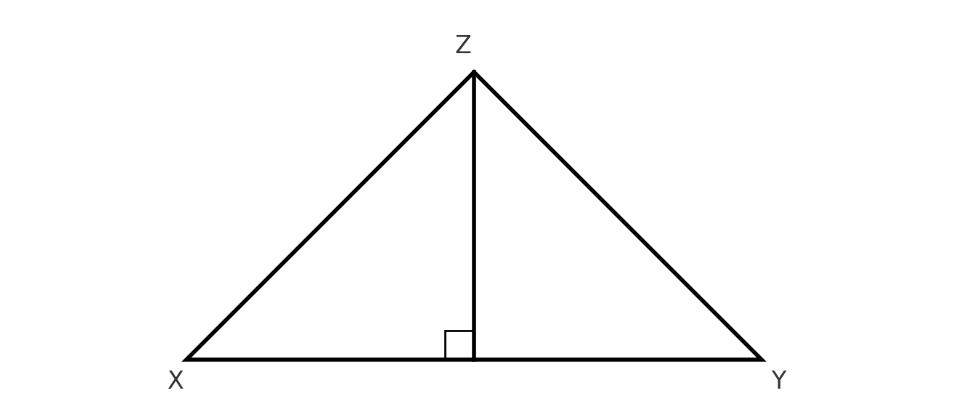
\includegraphics[width=0.5\linewidth]{hard_2_f1.png}
\end{center}

In the figure shown, the measure of angle \(Y\) is \(38^\circ\). The length of \(XY\) is 12 meters, and the length of \(YZ\) is 5 meters. What is the area, in square meters, of triangle \(XYZ\)?
\vspace{0.35cm}
\begin{enumerate}
    \item[A.] 30
    \item[B.] 60
    \item[C.] \(30 \sin 38^\circ\)
    \item[D.] \(60 \sin 38^\circ\)
\end{enumerate}
\end{frame}
\begin{frame}{Answer 1}
\small
\textbf{Correct Answer:} C
\end{frame}

% --- Question 2 ---
\begin{frame}{Question 2}
\small
A research manager selected two random samples to estimate the average lifespan of a certain type of light bulb (in hours). Based on the first sample, the research manager estimated that the average lifespan of this type of light bulb is 800 hours, with a margin of error of 20 hours.

Based on the second sample, the research manager estimated that the average lifespan of this type of light bulb is 810 hours, with a margin of error of 35 hours.

Assuming the margins of error were calculated in the same way, which of the following best explains why the first sample obtained a smaller margin of error than the second sample?
\vspace{0.35cm}
\begin{enumerate}
    \item[A.] The first sample contained fewer light bulbs than the second sample.
    \item[B.] The first sample contained more light bulbs than the second sample.
    \item[C.] The first sample had a shorter average lifespan than the second sample.
    \item[D.] The first sample had a longer average lifespan than the second sample.
\end{enumerate}
\end{frame}
\begin{frame}{Answer 2}
\small
\textbf{Correct Answer:} B
\end{frame}

% --- Question 3 ---
\begin{frame}{Question 3}
\small
The function \(p(x)\) is defined by:
\[
p(x) = a((x - 3)^2 + b)((x - 3)^2 - c),
\]
where \(a, b,\) and \(c\) are constants. The graph of \(y = p(x)\) passes through the points \((1, 25)\) and \((-1, 52)\).

What is the value of \(p(5) + p(7)\)?
\vspace{0.35cm}
\begin{enumerate}
    \item[A.] 25
    \item[B.] 27
    \item[C.] 52
    \item[D.] 77
\end{enumerate}
\end{frame}
\begin{frame}{Answer 3}
\small
\textbf{Correct Answer:} D
\end{frame}

% --- Question 4 ---
\begin{frame}{Question 4}
\small
In the given function, \(b\) is a positive constant. For every increase in the value of \(x\) by 1, the value of \(f(x)\) increases by \(c\%\), where \(0 < c < 100\).

Which expression gives the value of \(c\) in terms of \(b\)?
\[
f(x) = 77(b)^x
\]
\vspace{0.35cm}
\begin{enumerate}
    \item[A.] \(1 + \dfrac{b}{100}\)
    \item[B.] \(b + 100\)
    \item[C.] \(100(b + 1)\)
    \item[D.] \(100(b - 1)\)
\end{enumerate}
\end{frame}
\begin{frame}{Answer 4}
\small
\textbf{Correct Answer:} D
\end{frame}

% --- Question 5 ---
\begin{frame}{Question 5}
\small
On average, a certain tree grows 87 centimeters every \(m\) months. At this rate, which expression represents the number of centimeters, on average, the tree grows every \(k\) years?
\vspace{0.35cm}
\begin{enumerate}
    \item[A.] \(\dfrac{29m}{4k}\)
    \item[B.] \(\dfrac{29k}{4m}\)
    \item[C.] \(\dfrac{1044m}{k}\)
    \item[D.] \(\dfrac{1044k}{m}\)
\end{enumerate}
\end{frame}
\begin{frame}{Answer 5}
\small
\textbf{Correct Answer:} D
\end{frame}

% --- Question 6 ---
\begin{frame}{Question 6}
\small
\begin{center}
    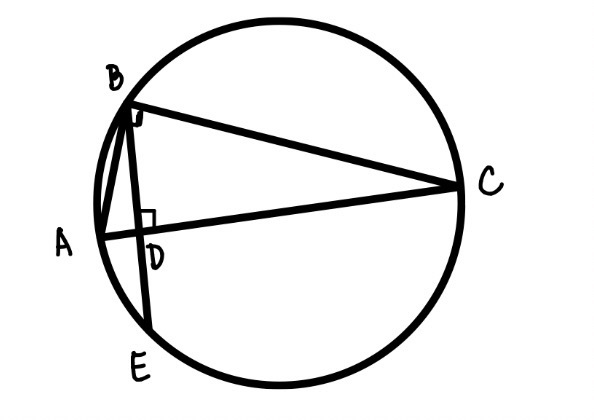
\includegraphics[width=0.5\linewidth]{hard_2_f2.jpg}
\end{center}

In the figure shown, points \(A, B, C,\) and \(E\) lie on the circle, and \(AB < BC\). Segment \(AC\) is perpendicular to segment \(BE\) at point \(D\), and \(BD = \sqrt{346}\). The diameter of the circle is 175. If \(\dfrac{CD}{AD} = r\), what is the value of \(r\)?
\end{frame}
\begin{frame}{Answer 6}
\small
\textbf{Final Answer:} $\boxed{86.5}$
\end{frame}

% --- Question 7 ---
\begin{frame}{Question 7}
\small
In the given equation, \(a\) and \(k\) are constants, where \(k > 5a\). The sum of the solutions to the equation is \(3k + 32\). What is the value of \(a\)?
\[
(x - k)^2 = (k - 5a)(x - k)
\]
\vspace{0.35cm}
\begin{enumerate}
    \item[A.] \(-\dfrac{32}{5}\)
    \item[B.] \(\dfrac{32}{5}\)
    \item[C.] \(-\dfrac{5}{32}\)
    \item[D.] \(\dfrac{5}{32}\)
\end{enumerate}
\end{frame}
\begin{frame}{Answer 7}
\small
\textbf{Correct Answer:} A
\end{frame}

% --- Question 8 ---
\begin{frame}{Question 8}
\small
The equation \(N(m) = 63(Q)^{m/6}\) gives the predicted population \(N(m)\), in thousands, of a certain bacteria colony \(m\) minutes after the initial measurement, where \(Q\) is a constant greater than 1. The predicted population increases by \(p\%\) every 180 seconds.

What is the value of \(p\) in terms of \(Q\)?
\vspace{0.35cm}
\begin{enumerate}
    \item[A.] \(100(Q^{30} - 1)\)
    \item[B.] \(100(Q^{\frac{1}{2}} - 1)\)
    \item[C.] \(100(Q^{30} + 1)\)
    \item[D.] \(100(Q^{1.5} + 1)\)
\end{enumerate}
\end{frame}
\begin{frame}{Answer 8}
\small
\textbf{Correct Answer:} B
\end{frame}

% --- Question 9 ---
\begin{frame}{Question 9}
\small
In the given equation, \(m\) and \(n\) are constants. The sum and product of the solutions of the equation are 8 and \(\dfrac{7}{2}\), respectively.

What is the value of \(\dfrac{m}{n}\)?
\[
(x - m)^2 = (m + 2n)(2x - n)
\]
\vspace{0.35cm}
\begin{enumerate}
    \item[A.] \(-\dfrac{1}{3}\)
    \item[B.] \(\dfrac{1}{3}\)
    \item[C.] -3
    \item[D.] 3
\end{enumerate}
\end{frame}
\begin{frame}{Answer 9}
\small
\textbf{Correct Answer:} D
\end{frame}

\begin{frame}{}
    \begin{tikzpicture}[remember picture, overlay]
        \shade[top color=novelPurple!40, bottom color=white]
            (current page.north west) rectangle (current page.south east);
        \fill[white, opacity=0.15] (current page.center) circle (5cm);
        \foreach \x in {1,2,3,4,5} {
            \fill[novelPurple, opacity=0.12] (rand*10-5, rand*7-3.5) circle (0.1+\x*0.05);
        }
    \end{tikzpicture}
    \centering
    \vspace{5em}
    {\Huge \textbf{\textcolor{novelPurple}{Thank You!}}} \\[1em]
    {\large \textcolor{gray}{We appreciate your time and focus.}} \\[3em]
    {\LARGE \textbf{\textcolor{novelPurple}{\textsf{Novel Prep}}}}
    \vfill
\end{frame}

\end{document}
